\documentclass{article}
\usepackage{amsmath}

\title{Simple Bayesian burst finding}
\author{Ben Gamari}

\newcommand{\lburst}{\ensuremath{\lambda_\mathrm{Burst}}}
\newcommand{\lbg}{\ensuremath{\lambda_\mathrm{BG}}}

\begin{document}
\maketitle

The algorithm makes use of the property of temporal locality of
bursts, e.g. a burst photon at time $t$ means a photon at time $t +
\Delta t$ is also likely due to the same burst. This property arises
when the characteristic diffusion time of the sample specimen is 
longer than the expected photon interarrival time.

The general idea behind the model is to examine a photon $i$ in
conjunction with the $N$ photons preceding and succeeding it. By
examining the interarrival times between these photons, we can infer
from which of two distributions, background or burst, the window of
photons was drawn.

The model likelihood for a photon $j$ is given by,
\begin{equation}
  L_j = \prod_{i=j-N}^{j+N} \sum_{s\in\{\mathrm{Burst}, \mathrm{BG}\}} P(\tau_i \vert \lambda_s) P(B_i = s)
\end{equation}
This can be evaluated independently for each photon.

Under this model, we can test the two hypotheses $B_i =
\mathrm{Burst}$ and $B_i = \mathrm{BG}$ for each photon. Specifically,
we can compute a Bayes factor $\beta$,
\begin{equation}
  \beta_i = \frac{P(\tau_i \vert \lburst)}{P(\tau_i \vert \lbg)}
\end{equation}
which represents the certainty of the model in one hypothesis over the
other. With reasonable settings of parameters $\lburst, \lbg$, the
Bayes factor is extremely sensitive to the temporal locality of our
bursts. The final inferred values of $B_i$ are decided by simple
thresholding of $\beta_i$. A reasonable threshold is 2.

\begin{figure}
\centering
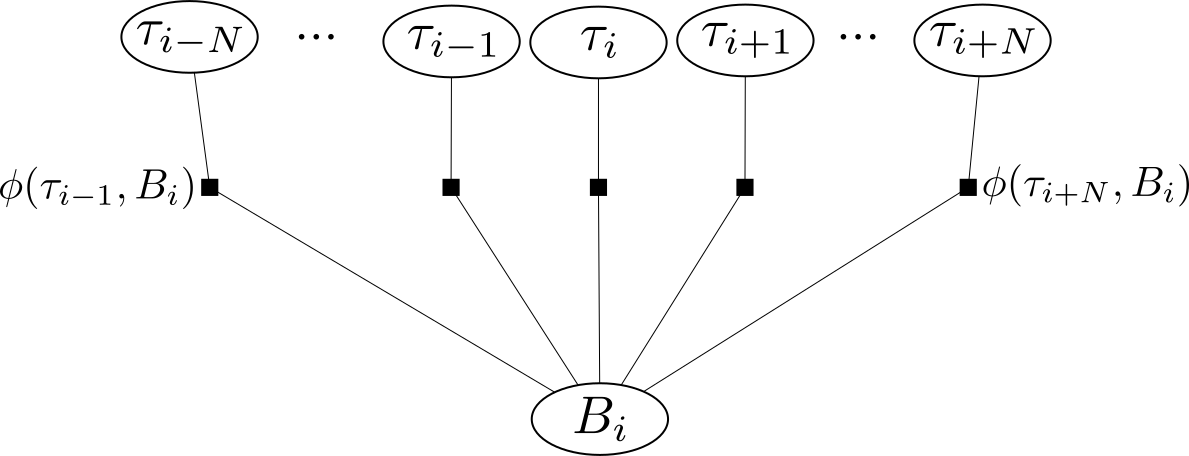
\includegraphics[scale=0.35]{burst-model.pdf}
\caption{The factor graph representation of the Bayesian burst-finding
algorithm. Here, $\tau$ denotes a photon inter-arrival time. $B_i$ is
a boolean variable indicating whether photon $i$ is due to a
burst. Note that the nodes $\tau_{i-N+1} ... \tau_{i-2}$ and
$\tau_{i+2} ... \tau_{i+N-1}$ have been omitted for consiseness.}
\end{figure}

\begin{equation}
  \phi(\tau, B) = \left\{
    \begin{array}{l l}
      P(\tau \vert \lambda_\mathrm{Burst})  & B = \mathrm{Burst} \\
      P(\tau \vert \lambda_\mathrm{BG})     & B = \mathrm{BG} \\
    \end{array}
  \right.
\end{equation}
where $P(\tau \vert \lambda)$ is given by the standard exponential
distribution, giving the distribution over interarrival times of a
homogenous Poisson process,
\[ P(\tau \vert \lambda) = \lambda e^{-\tau \lambda} \]

\end{document}
